\documentclass{article}

% Recommended, but optional, packages for figures and better typesetting:
\usepackage{microtype}
\usepackage{graphicx}
\usepackage{subfigure}
\usepackage{booktabs} 
\usepackage{hyperref}
\usepackage{amsmath}
\usepackage{amssymb}

\newcommand{\theHalgorithm}{\arabic{algorithm}}

\usepackage[accepted]{icml2021}

\icmltitlerunning{Highway Autonomous Driving via Deep Reinforcement Learning}

\begin{document}

\twocolumn[
\icmltitle{Highway Autonomous Driving via Deep Reinforcement Learning}

\icmlsetsymbol{equal}{*}

\begin{icmlauthorlist}
\icmlauthor{Edoardo Furlan}{}
\end{icmlauthorlist}

\icmlkeywords{Reinforcement Learning, Autonomous Driving, DQN, HighwayEnv}

\vskip 0.3in
]

\printAffiliationsAndNotice{} 

\begin{abstract}
This report explains the results obtained from the application of deep reinforcement learning algorithms for autonomous vehicle control in a highway scenario using the \texttt{HighwayEnv} simulator. I first define the kinematics of the problem and compare a simple DQN network against a deterministic and a human baseline. Then, to improve the performances of the first trained network, I modify different parameters such as reward function and network's structure in order to determine how these aspects contribute to the overall behaviour of the agent.
\end{abstract}

\section{Introduction to the Problem}

Highway autonomous driving is an overall very complex task for the agent. In this scenario the environment poses a great challenge due to the many kind of unknown variables from the surrounding: the goal is then to quickly adapt to different conditions while maintaining the driving objectives like speed and desired lane. To simulate the environment, in this work I employ the \texttt{highway-v0} environment from the \texttt{HighwayEnv} simulator \cite{highway-env}.
\subsection{State Space}
The state observed by the agent at each time step is represented by a $V \times F$ matrix of size $5 \times 5$, describing the state of the vehicle and the $4$ nearest surrounding vehicles. Notice that the scene may contain more vehicles, but only the closest four are considered by the agent. The features ($F = 5$) provided for each vehicle are:
\begin{itemize}
    \item \textbf{Presence}: A binary value ($0$ or $1$) indicating the actual presence of the vehicle.
    \item \textbf{$x$}: Longitudinal position relative to the ego-vehicle.
    \item \textbf{$y$}: Lateral position relative to the ego-vehicle.
    \item \textbf{$v_x$}: Longitudinal velocity relative to the ego-vehicle.
    \item \textbf{$v_y$}: Lateral velocity relative to the ego-vehicle.
\end{itemize}

The first row of the matrix contains the features of the ego-vehicle in absolute coordinates, whereas the subsequent rows describe the surrounding vehicles in relative coordinates with respect to the ego-vehicle.

\subsection{Action Space}
The agent interacts with the environment through a discrete action space consisting of $5$ possible actions:
\begin{enumerate}
    \setcounter{enumi}{0}
    \item \textbf{LANE LEFT}: Change lane to the left.
    \item \textbf{IDLE}: Maintain the current lane and speed.
    \item \textbf{LANE RIGHT}: Change lane to the right.
    \item \textbf{FASTER}: Accelerate.
    \item \textbf{SLOWER}: Decelerate.
\end{enumerate}

\subsection{Default Reward Function}
The original reward function provided by the environment is defined as a linear combination of three main terms:
\begin{equation}
    R = a \cdot R_{speed} + b \cdot R_{right} + c \cdot R_{collision}
\end{equation}
where $a$, $b$, and $c$ represent the weights of each component (by default, $a=0.4$, $b=0.1$, and $c=-1.0$), and:
\begin{itemize}
    \item $R_{speed}$ is the speed reward, calculated linearly within the specified speed range $[20, 30]$ m/s.
    \item $R_{right}$ is the right-lane reward, rewarding the agent for occupying the rightmost lanes.
    \item $R_{collision}$ is a binary indicator of collision ($1$ if a collision occurs, $0$ otherwise).
\end{itemize}

\section{Baseline Policy and Manual Control}
To evaluate the RL agent's performance, I compare it against two primary benchmarks:
\begin{itemize}
    \item \textbf{Manual Control (Human)}: I manually controlled the vehicle using the keyboard. This establishes the empirical upper bound of performance for a driver balancing high speeds and efficient lane changes.
    \item \textbf{Rule-Based Heuristic (Advanced Baseline)}: I designed a deterministic controller that uses the state matrix as a guide to detect and avoid obstacles. The controller checks for obstacles by analyzing relative distance and velocity thresholds: a front obstacle is detected if a vehicle is within a short range ($0 < x < 0.1$, corresponding to normalized distance) with a negative relative speed ($v_x < 0$), indicating a potential incident. Similarly, left and right neighboring spaces are monitored for vehicle presence within lateral boundaries ($-0.45 < y < -0.2$ and $0.2 < y < 0.45$, respectively). The decision logic prioritizes steering maneuvers to bypass congestion: if the path ahead is blocked, it steers to the right lane if clear, otherwise to the left lane, and decelerates only if both options are blocked. If the front path is clear, it prioritizes returning to the rightmost lane to maximize the traffic flow reward, and accelerates to maintain speed.
\end{itemize}

\section{Deep Q-Network (DQN) Agent}
The reinforcement learning agent implements the standard Deep Q-Network (DQN) algorithm \cite{mnih2015human} with the following details:

\subsection{Architecture and Hyperparameters}
The model approximates the action-value function $Q(s, a)$ using a multi-layer perceptron (MLP) consisting of three linear layers:
\begin{itemize}
    \item \textbf{Input Layer}: 25 nodes (flattened $5 \times 5$ state matrix).
    \item \textbf{Hidden Layers}: Two linear layers with $128$ and $64$ neurons, respectively, each followed by a ReLU activation function.
    \item \textbf{Output Layer}: $5$ linear nodes representing the Q-values for the $5$ discrete actions.
\end{itemize}

Training is conducted using a Replay Buffer with a capacity of $15,000$ transitions, from which mini-batches of size $64$ are sampled. The discount factor is set to $\gamma = 0.99$. To ensure stability, the target network is updated softly (\textit{soft update}) at each optimization step with a parameter $\tau = 0.005$. The exploration policy is $\epsilon$-greedy with a linear decay of $\epsilon$ from $1.0$ to $0.05$ over the first $5,000$ training steps. The optimizer is Adam with a learning rate of $5 \cdot 10^{-4}$.

\section{Initial Results}
All models were tested over $10$ independent episodes in the standard \texttt{highway-v0} environment (3 lanes, ego spacing of 1.5). Table~\ref{tab:initial-results} reports the average metrics.

\begin{table}[ht]
\caption{Comparison of average performance over 10 evaluation episodes.}
\label{tab:initial-results}
\vskip 0.15in
\begin{center}
\begin{small}
\renewcommand{\arraystretch}{1.3}
\setlength{\tabcolsep}{3pt}
\begin{tabular}{lccccc}
\toprule
Agent & Return & Length & Crash & Lane Ch. & Speed \\
 & & (Steps) & (\%) & (Count) & (m/s) \\
\midrule
Human & 37.21 & 38.50 & 10.0\% & 11.80 & 29.28 \\
DQN Base & 27.82 & 40.00 & 0.0\% & 22.10 & 20.03 \\
Advanced Baseline & 23.01 & 23.20 & 80.0\% & 5.80 & 27.02 \\
\bottomrule
\end{tabular}
\end{small}
\end{center}
\vskip -0.1in
\end{table}

\subsection{Analysis of Results}
The analysis of the experimental data highlights the following key points:
\begin{itemize}
    \item \textbf{Base DQN} achieves exceptional safety with a $0\%$ crash rate. However, this safety is the result of a very cautious driving style: the agent never accelerates, maintaining an average speed of $20.03$ m/s which is indeed very close to the minimum allowed speed. Additionally, the policy is laterally unstable, resulting in $22.1$ lane changes per episode (zig-zagging constantly). The results indicate that the network is able to avoid collisions but at the expense of an extremely safe driving style.
    \item \textbf{The Advanced Baseline} travels fast ($27.02$ m/s) and makes few lane changes ($5.8$), but is highly vulnerable, registering an $80\%$ crash rate. This indicates that the deterministic behaviour is not well suited to determine a driving style that is able to adapt to every scenario.
    \item \textbf{Human Control} demonstrates that it is possible to combine high speeds ($29.28$ m/s) and stability ($11.8$ lane changes) while keeping crashes minimal (10\%).
\end{itemize}

The results show that a simple DQN network is actually able to perform better than a deterministic policy, but to reach a human level performance many other adjustments need to be made. This performance gap motivates the reward shaping techniques and network architecture modifications (Double DQN) detailed in the next section.

\section{Bonus Enhancements}
In order to bridge the gap with human performance, I explored several bonus modifications in a structured progression. For each phase, I present an initial attempt, identify its failure modes, and apply a targeted refinement. Importantly, I maintain the testing environment completely standard (evaluating on the original reward function) to ensure a fair comparison. Table~\ref{tab:standard-dqn-results} reports the average metrics for the standard DQN variations (Phases 1--3), while Table~\ref{tab:ddqn-results} reports the performance of the Double DQN configurations (Phase 4).

The primary limitation of the baseline DQN agent is its overly conservative driving style and high lateral instability. These issues stem from:
\begin{itemize}
    \item \textbf{Reward misalignment}: The default reward function does not penalize frequent lane changes, leading to constant zig-zagging, and does not discourage tailgating.
    \item \textbf{State representation limits}: The standard flattened $5 \times 5$ kinematics grid lacks direct spatial and safety context, forcing the network to guess lane layouts and safety margins. This suggests that enriching the state representation may be helpful to give the network more context and improve training efficiency.
    \item \textbf{Environment mismatch}: The agent is trained on a 4-lane setup (standard environment from the library) but evaluated on a denser 3-lane scenario.
    \item \textbf{Network's Architecture}: The standard DQN architecture can be enriched in order to improve its performance.
\end{itemize}

\subsection{Reward Function Modification}
To align the agent's objective with new specifications, I use a function that modifies the reward function used internally by the agent during training. This is done by adding penalty terms to the baseline feedback to discourage frequent lane changes and dangerous tailgating. Crucially, this shaped reward is only used internally during the training phase to guide policy learning; during testing and evaluation, the agent is evaluated using the completely standard, unmodified environment reward function ($R_{env}$) to guarantee a fair comparison. I define the shaped reward function $R_{\text{shaped}}$ as:
\begin{equation}
\begin{split}
    R_{\text{shaped}} = & \, R_{env} - \beta \cdot R_{\text{proximity}} \\
    & - \alpha \cdot \mathbb{I}(a \in \mathcal{A}_{\text{steer}})
\end{split}
\end{equation}
where $R_{env}$ is the original environment reward, $\alpha = 0.15$ is the penalty for steering actions, $\mathcal{A}_{\text{steer}} = \{\text{LANE\_LEFT}, \text{LANE\_RIGHT}\}$ is the set of steering actions, and the proximity penalty $R_{\text{proximity}} = \max\left(0, \frac{d_{safe} - d_{lead}}{d_{safe}}\right)$ triggers when the normalized distance $d_{lead}$ to the leading vehicle in the same lane falls below $d_{safe}$, with a penalty weight of $\beta = 0.30$. I compare two configurations:
\begin{itemize}
    \item \textbf{P1.1: Shape (Weak)}: Initial configuration with a narrow safety distance $d_{safe} = 0.20$. This model yields a return of $28.24$ and reduces lane changes (from $22.10$ down to $11.30$), but still suffers from a $10.0\%$ crash rate because the proximity margin was too small.
    \item \textbf{P1.2: Shape (Strict)}: Refinement with a wider safety distance $d_{safe} = 0.25$. This model completely resolves the safety issue, achieving a $0.0\%$ crash rate and $100\%$ survival. However, the agent remains highly conservative, maintaining a minimum speed of $20.04$ m/s.
\end{itemize}

Additionally, I investigated the effect of a slower exploration decay ($\epsilon$-decay over 10,000 steps instead of 5,000) under the strict reward shaping configuration. The idea is to provide more exploration an hopefully better results. However I obtained no significant improvements in this phase: the agent's speed remained close to the minimum limit while still registering minor collision risks, indicating that reward shaping alone is insufficient to learn a high-speed and more courageous policy.


\subsection{Environment Configuration Changes}
By default, the training environment (\texttt{highway-fast-v0}) has 4 lanes, while the evaluation setup has only 3 lanes. This mismatch in road geometry (where 3 lanes are much denser and leave less room for steering maneuvers) creates a significant generalization gap. To resolve this, in \textbf{P2: Env Config}, I trained the agent directly on a 3-lane highway layout (incorporating the strict shaped reward from Phase 1.2). Matching the training environment structure with the evaluation setup allows the agent to learn steering and deceleration behaviors optimized for narrower traffic, yielding a return of $28.64$, a $0.0\%$ crash rate, and a stable steering policy ($8.00$ lane changes).

Again however the agent remained very conservative.

\subsection{State Representation Modification}
To allow the agent to speed up safely, I enrich the state representation. The idea is to provide it with more information about the environment in order to allow it to make smarter decisions. I design a new representation (\textbf{P3: State Mod}) that appends 4 new features to the kinematics matrix (resulting in a 29-dimensional state): the ego absolute lane index, the Time-to-Collision (TTC) to the leading vehicle, and clearances in the left and right adjacent lanes. 

The absolute lane index allows the network to map lane coordinates, removing the need of having to guess its lane position from the raw $y$ data. The Time-to-Collision is calculated as:
\begin{equation}
    \text{TTC} = \frac{\Delta x}{|\Delta v_x|}
\end{equation}
providing a direct warning of incoming collisions. Left and right clearances monitor neighboring lanes, acting as safety indicators for lateral maneuvers. I compared two training settings:
\begin{itemize}
    \item \textbf{P3.1: State (Short Exp)}: Trained with the default fast exploration decay ($\epsilon$-decay over $5,000$ steps). The agent is safe ($0.0\%$ crashes) and speeds up slightly ($20.38$ m/s), but remains overly cautious.
    \item \textbf{P3.2: State (Long Exp)}: Trained with a longer exploration phase ($\epsilon$-decay over $10,000$ steps) to allow the agent to discover high-speed rewards under safety clearances. This results in a massive improvement in lateral stability (reducing lane changes to a mere $1.20$) and a slight speed increase to $20.69$ m/s (peaking at $22.28$ m/s). However, driving faster under standard DQN introduces a $10.0\%$ crash rate probably due to unstable Q-value estimates.
\end{itemize}

\begin{figure}[ht]
\centering
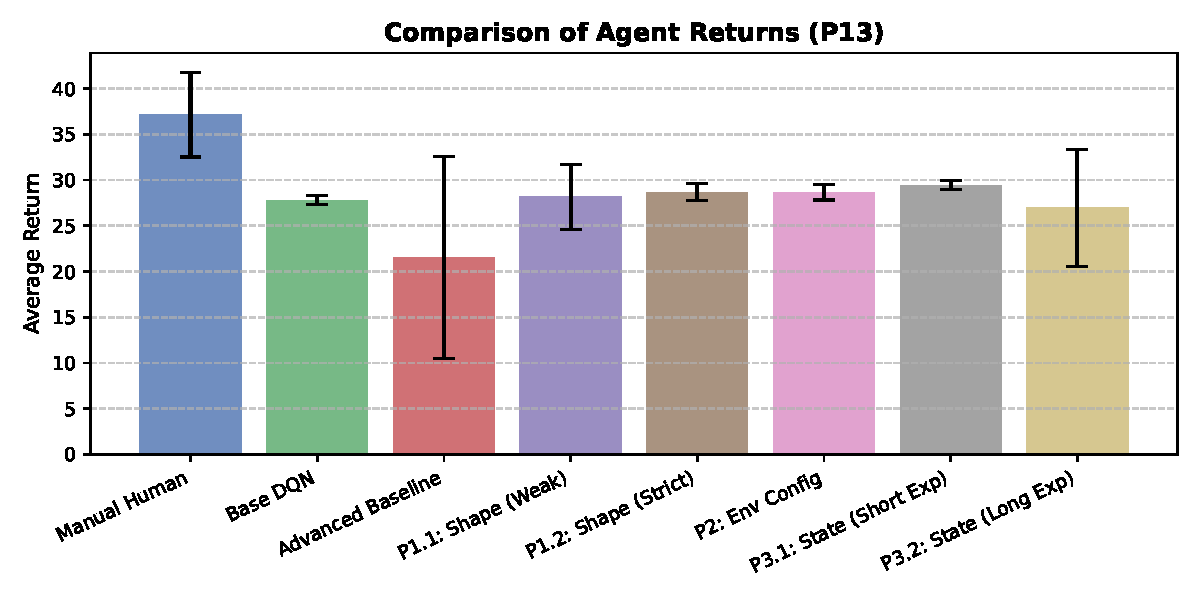
\includegraphics[width=0.95\columnwidth]{../rl_project_ad/plot_data/comparison_returns_p13.pdf}
\caption{Average episode returns comparison for standard DQN variations (Phases 1-3).}
\label{fig:returns_p13}
\end{figure}

\begin{figure}[ht]
\centering
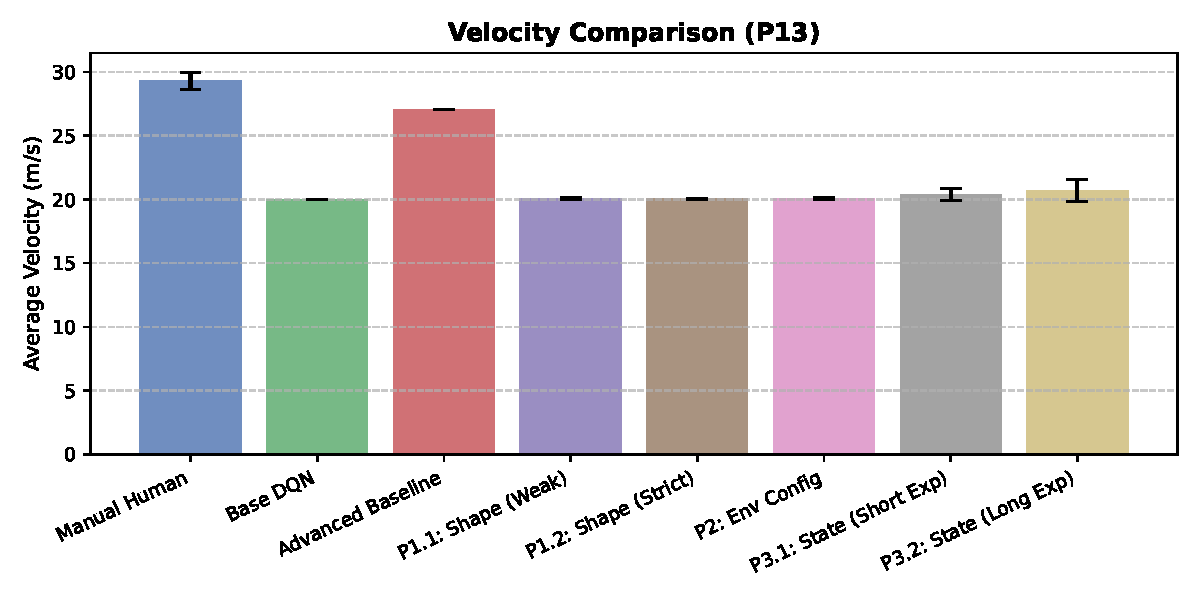
\includegraphics[width=0.95\columnwidth]{../rl_project_ad/plot_data/comparison_velocities_p13.pdf}
\caption{Average velocity comparison for standard DQN variations (Phases 1-3).}
\label{fig:velocities_p13}
\end{figure}

\begin{table}[ht]
\caption{Comparison of average performance for standard DQN variations (Phases 1--3) over 10 evaluation episodes.}
\label{tab:standard-dqn-results}
\vskip 0.15in
\begin{center}
\begin{small}
\renewcommand{\arraystretch}{1.3}
\setlength{\tabcolsep}{2pt}
\begin{tabular}{lccccc}
\toprule
Configuration & Return & Length & Crash & Lane Ch. & Speed \\
 & & (Steps) & (\%) & (Count) & (m/s) \\
\midrule
Human & 37.21 & 38.50 & 10.0\% & 11.80 & 29.28 \\
DQN Base & 27.82 & 40.00 & 0.0\% & 22.10 & 20.03 \\
\midrule
P1.1: Shape (W) & 28.24 & 38.50 & 10.0\% & 11.30 & 20.07 \\
P1.2: Shape (S) & 28.66 & 40.00 & 0.0\% & 15.60 & 20.04 \\
\midrule
P2: Env Config & 28.64 & 40.00 & 0.0\% & 8.00 & 20.06 \\
\midrule
P3.1: State (Short Exp) & 29.43 & 40.00 & 0.0\% & 13.30 & 20.38 \\
P3.2: State (Long Exp) & 26.98 & 37.20 & 10.0\% & 1.20 & 20.69 \\
\bottomrule
\end{tabular}
\end{small}
\end{center}
\vskip -0.1in
\end{table}

\subsection{Algorithmic and Network Upgrades}
Finally, I upgraded the agent to a Double DQN architecture (\textbf{P4: Double DQN}) to address the overestimation of action-values. In standard DQN~\cite{mnih2015human}, the target Q-value update uses the target network parameters $\theta^-_t$ to both select the best action and estimate its value:
\begin{equation}
    Y^{\text{DQN}}_t = R_{t+1} + \gamma \max_{a} Q(S_{t+1}, a; \theta^-_t)
\end{equation}
This coupling leads to a systematic overestimation of Q-values due to the maximization bias, which was analyzed and resolved by Van Hasselt et al.~\cite{van2016deep} in their paper \textit{"Deep Reinforcement Learning with Double Q-Learning"}. 

Double DQN decouples action selection from action evaluation by selecting the greedy action using the online network parameters $\theta_t$, but evaluating its Q-value using the target network parameters $\theta^-_t$:
\begin{equation}
\begin{split}
    Y^{\text{DDQN}}_t = & \, R_{t+1} + \gamma Q\big(S_{t+1}, \\
    & \operatorname{argmax}_{a} Q(S_{t+1}, a; \theta_t); \theta^-_t\big)
\end{split}
\end{equation}
This formulation significantly mitigates optimistic Q-value bias, stabilizing training.

To evaluate the impact of this architectural upgrade, I established a starting baseline configuration. The initial Double DQN model was trained using the modified shaped reward function (from Phase 1) and the enriched 29-dimensional state representation (from Phase 3). For a direct comparison against the standard DQN models, I initially trained the agent on the default 4-lane road layout. This starting point allows me to isolate the effect of the network upgrade itself on driving velocity, before addressing road geometry matching. From this starting point, I iteratively evaluate five Double DQN configurations:
\begin{itemize}
    \item \textbf{P4.1: DDQN (4 Lanes)}: The initial Double DQN model trained on the default 4-lane layout but evaluated on the denser 3-lane scenario. This configuration demonstrates that the Double DQN network allows the agent to achieve a significantly higher velocity ($23.34$ m/s) compared to standard DQN; however, it remains highly accident-prone, suffering a $40.0\%$ crash rate.
    \item \textbf{P4.2: DDQN (3 Lanes)}: Resolving the layout mismatch by training directly on a 3-lane setup. This configuration achieves absolute safety ($0.0\%$ crash rate) and high return ($29.13$), but remains somewhat conservative with an average speed of $20.90$ m/s and very few lane changes ($2.50$).
    \item \textbf{P4.3: DDQN (Balanced)}: Trained with tuned trade-off parameters (safety distance $0.28$, proximity penalty $0.35$, speed reward $0.45$) to encourage higher velocity. Since the higher speed incentive caused a resurgence of rapid, consecutive lane changes, I introduced a zig-zag penalty ($\zeta = 0.25$) in the reward function when steering actions are taken within 4 steps of a previous one. The agent successfully drives at $22.25$ m/s with $0.0\%$ crashes. However, it displays a “lane-stickiness" behavior: when blocked by a slow vehicle while driving in the rightmost lane, it stays tailgating rather than performing a clean overtake because the lane change penalty ($-0.20$ total) is too high compared to the proximity penalty.
    \item \textbf{P4.4: DDQN (Tuned)}: A refined configuration to promote active overtaking and prompt return to the right-most lane. To achieve this, the right lane reward is increased to $0.20$ to incentivize returning to the right lane, while the total lane change penalty is kept moderate at $-0.12$ ($-0.06$ environment + $-0.06$ additional from internal function) to prevent aimless zig-zagging. Proximity parameters are kept at a safety distance of $0.25$ and penalty of $0.25$ to maintain a brave, close-driving style. This configuration achieves an average speed of $21.65$ m/s, $0.0\%$ crash rate, and very stable lane selection (averaging only $2.30$ lane changes per episode).
\end{itemize}

Figures~\ref{fig:returns_p4} and \ref{fig:velocities_p4} show the comparison of returns and average velocities for the Double DQN configurations (Phase 4).

\begin{figure}[ht]
\centering
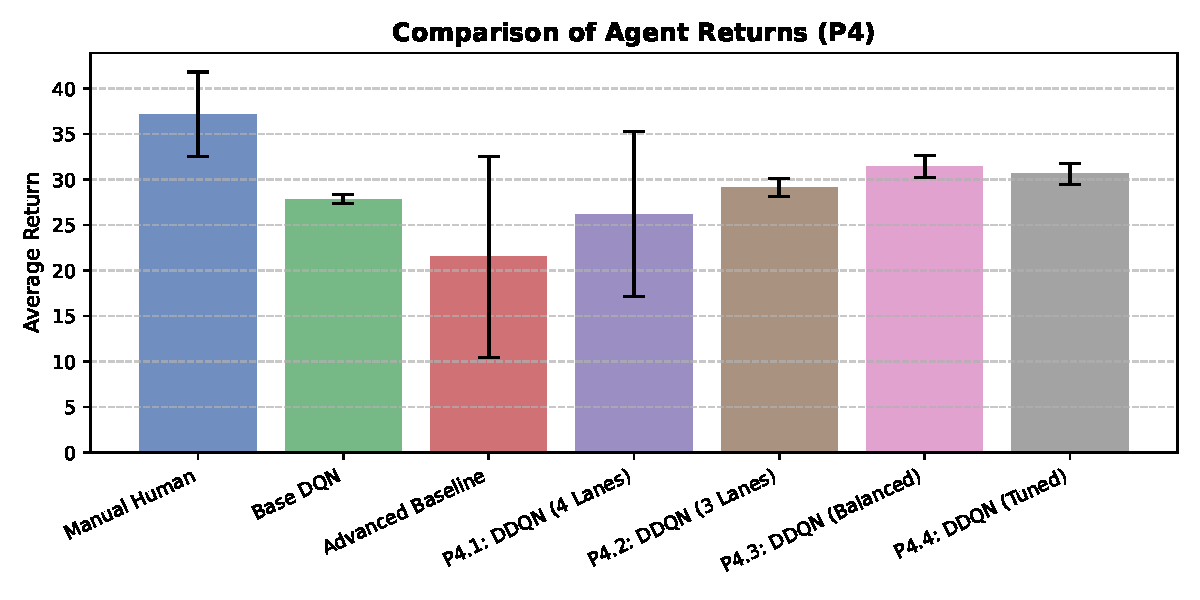
\includegraphics[width=0.95\columnwidth]{../rl_project_ad/plot_data/comparison_returns_p4.pdf}
\caption{Average episode returns comparison for Double DQN configurations (Phase 4).}
\label{fig:returns_p4}
\end{figure}

\begin{figure}[ht]
\centering
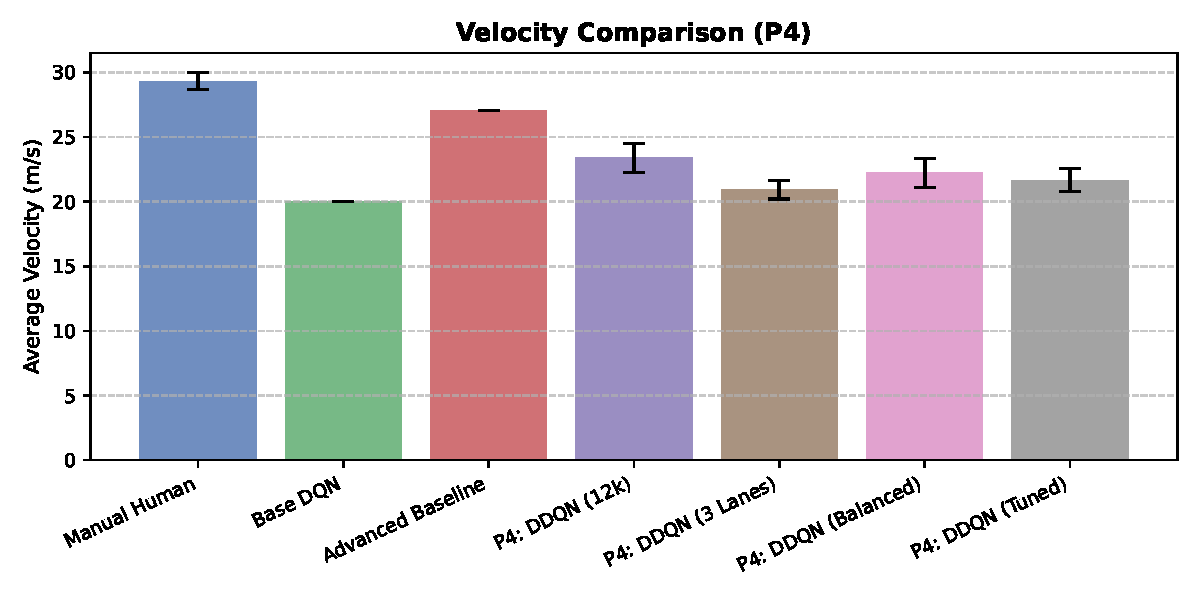
\includegraphics[width=0.95\columnwidth]{../rl_project_ad/plot_data/comparison_velocities_p4.pdf}
\caption{Average velocity comparison for Double DQN configurations (Phase 4).}
\label{fig:velocities_p4}
\end{figure}

\begin{table}[ht]
\caption{Comparison of average performance for Double DQN configurations (Phase 4) over 10 evaluation episodes.}
\label{tab:ddqn-results}
\vskip 0.15in
\begin{center}
\begin{small}
\renewcommand{\arraystretch}{1.3}
\setlength{\tabcolsep}{2pt}
\begin{tabular}{lccccc}
\toprule
Configuration & Return & Length & Crash & Lane Ch. & Speed \\
 & & (Steps) & (\%) & (Count) & (m/s) \\
\midrule
P4.1: DDQN (4 Lanes) & 26.17 & 32.80 & 40.0\% & 4.80 & 23.34 \\
P4.2: DDQN (3 Lanes) & 29.13 & 40.00 & 0.0\% & 2.50 & 20.90 \\
P4.3: DDQN (Balanced) & 31.38 & 40.00 & 0.0\% & 9.70 & 22.25 \\
P4.4: DDQN (Tuned) & 30.61 & 40.00 & 0.0\% & 2.30 & 21.65 \\
\bottomrule
\end{tabular}
\end{small}
\end{center}
\vskip -0.1in
\end{table}

\section{Conclusions}
In this project, I investigated the design of deep reinforcement learning policies for autonomous highway driving. Starting with the basic DQN agent, I addressed its safety and velocity limitations through a structured progression of reward shaping, environmental geometry matching, state representation enrichment, and algorithmic upgrades using Double DQN. 

My findings indicate that simple modifications to the vanilla DQN fail to provide the network enough context to improve its performing by making smart and brave decisions. Upgrading to Double DQN successfully decoupled action selection from evaluation, stabilizing training and allowing the network to learn a much higher-speed policy. By balancing the trade-offs between speed, right-lane preference, and lane change penalties in my final courageous configuration, I obtained a policy that actively and safely overtakes slower vehicles while promptly returning to the right-most lane, achieving high returns and a $0\%$ crash rate.
By improving architecture and fine tuning parameters, the network may be able to learn more proactive behavours and close the gap to the human baseline.

\bibliography{report}
\bibliographystyle{icml2021}

\end{document}
